\documentclass{beamer}
\usetheme[titleformat=regular,sectiontitleformat=regular,frametitleformat=regular]{m}

\usepackage[brazil]{babel}
\usepackage[numberedbib]{apacite}
\usepackage[utf8]{inputenc}

\title{Apresentação de artigo: A Genetic Programming Approach to Record Deduplication}
\date{\today}
\author{Herberth Amaral}
\institute{Programa de Pós-Graduação em Modelagem Computacional e Sistemas - UNIMONTES}
\begin{document}
  \maketitle

  \section{Introdução}

  \begin{frame}{Record linkage}
      \textit{Record linkage} (RL) é o processo de encontrar registros duplicados que representam a mesma entidade em um ou mais conjuntos de dados \cite{survey}.

      Faz parte das tarefas de \textit{data cleaning} dos processos de mineração de dados.
  \end{frame}

  \section{Teoria de RL}

  \begin{frame}{Modelagem matemática}
      Modelo desenvolvido por \cite{fellegi69}. Foi a primeira tentativa bem sucedida de criar um modelo matemático para RL.

      Compreende três decisões: \textit{link} ($A_1$), \textit{non-link} ($A_3$) e \textit{potential link} ($A_2$). Dois tipos de erro (para $A_1$ e $A_3$) também são definidos, respectivamente, da seguinte forma:

      \begin{center}
          $\mu = \sum\limits_{\gamma \in \Gamma} u(\gamma)P(A_1|\gamma)$ \\
          $\lambda = \sum\limits_{\gamma \in \Gamma} m(\gamma)P(A_3|\gamma)$
      \end{center}
  \end{frame}
  \begin{frame}{Modelagem matemática}

      Em que $\gamma$ é um vetor de comparações entre duas tuplas. $u(\gamma)$ e $m(\gamma)$ são probabilidades de realização de $\gamma$. O somatório é feito sobre todo o espaço de comparação $\Gamma$ de possíveis pares.

      Uma regra de ligação ótima $L(\mu,\lambda,\Gamma)$ associa as probabilidades $P(A_1|\gamma)$, $P(A_2|\gamma)$ e $P(A_3|\gamma)$ para cada uma das realizações de $\gamma$ de forma a minimizar $P(A_2)$.

  \end{frame}

  \begin{frame}{Programação genética}
      Programação evolucionária é baseada em idéias inspiradas do processo que influencia virtualmente todos os seres vivos, a \textit{seleção natural} \cite{geneticrl}.

      Programação gentética (GP) é uma das técnicas mais conhecidas dentro da programação evolucionária. Pode ser visto como uma heurística adaptativa em que as idéias básicas vem das propriedades das operações genéticas e seleção natural.

      A principal diferença entre GP e outras técnicas evolucionárias é que GPs representam o conceito do problema como um programa de computador. Ou seja, cada indivíduo é uma \textbf{\textit{função}}, representado como uma \textbf{\textit{árvore}}.
  \end{frame}
  \begin{frame}{Programação genética - algoritmo básico}
      \begin{enumerate}
          \item Inicialize a população;
          \item Avalia todos os indivíduos, associando uma nota (\textit{fitness}) a cada um;
          \item Execute o último passo se o critério de parada for atingido. Do contrário, continue;
          \item \textbf{Selecione} os melhores $n$ indivíduos para a próxima geração;
          \item Aplique os operadores de \textbf{cruzamento} e \textbf{mutação} para obter $m$ novos indivíduos;
          \item Substitua a população atual pela população gerada ao passo 2;
          \item Apresente o melhor indivíduo na população como saída do processo evolucionário.
      \end{enumerate}
  \end{frame}
  \begin{frame}{Programação genética - Operadores}
      Programação genética, assim como demais algoritmos evolucionários, possuem métodos para representar o procsso evolutivo:
      \begin{enumerate}
          \item Seleção;
          \item Cruzamento;
          \item Mutação;
      \end{enumerate}
  \end{frame}

  \begin{frame}{Programação genética - Seleção}
      É a operação que copia os indivíduos sem os modificar. Geralmente é feito com uma estratégia elitista, que mantém os melhores indivíduos para a próxima geração.
  \end{frame}

  \begin{frame}{Programação genética - Cruzamento}
      Permite que material genético (ou seja, sub-árvores) seja trocado entre dois pais em um processo que pode gerar um ou mais filhos. Os filhos são o resultado da troca das sub-árvores selecionadas entre os pais, conforme ilustrado na figura \ref{fig:crossover}.
      \begin{figure}
          \centering
          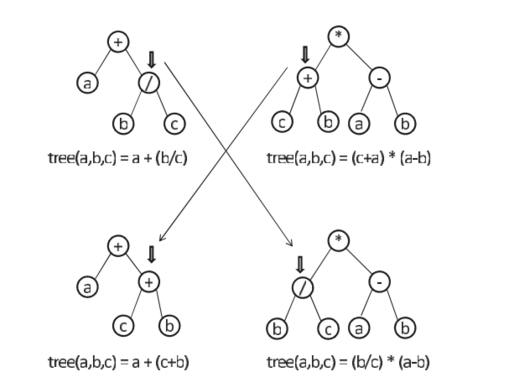
\includegraphics[width=0.4\textwidth]{crossover.png}
          \caption{Cruzamento entre árvores \cite{geneticrl}}
          \label{fig:crossover}
      \end{figure}
  \end{frame}

  \begin{frame}{Programação genética - Cruzamento}
      Permite que material genético (ou seja, sub-árvores) seja trocado entre dois pais em um processo que pode gerar um ou mais filhos. Os filhos são o resultado da troca das sub-árvores selecionadas entre os pais, conforme ilustrado na figura \ref{fig:crossover}.
      \begin{figure}
          \centering
          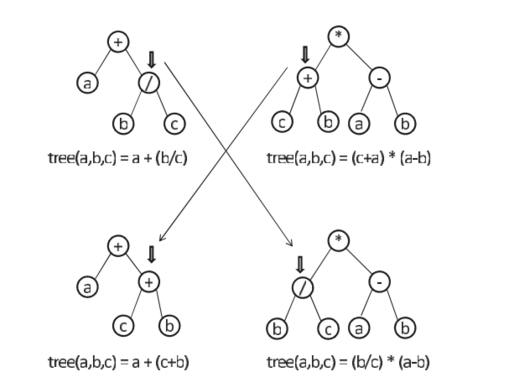
\includegraphics[width=0.4\textwidth]{crossover.png}
          \caption{Cruzamento entre árvores \cite{geneticrl}}
          \label{fig:crossover}
      \end{figure}
  \end{frame}

  \begin{frame}{Programação genética - Mutação}
      O operador de mutação possui o papel de aumentar a diversidade e, assim, fazer com que o PG explore melhor seu espaço de busca. Todos os indivíduos tem uma chance fixa de sofrer mutação. Numa árvore GP, um nó aleatório é selecionado e a sub-árvore correspondente é trocada por uma aleatoriamente criada, conforme ilustrado na figura \ref{fig:mutacao}.
      \begin{figure}
          \centering
          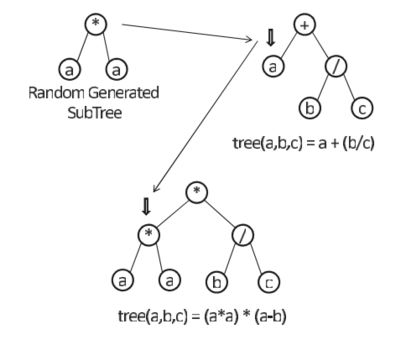
\includegraphics[width=0.4\textwidth]{mutacao.png}
          \caption{Mutação de sub-árvore \cite{geneticrl}}
          \label{fig:mutacao}
      \end{figure}
  \end{frame}

  \section{Modelando o problema de record linkage com programação genética}


  \section{Referências}
      \begin{frame}{Bibliography}
          \bibliographystyle{apacite}
          \bibliography{apresentacao}
      \end{frame}
\end{document}
